\documentclass[sigconf,anonymous,review]{acmart}
%% AISec @ CCS submission skeleton.
%% Build: see paper/README.md. Toggle `anonymous`/`review` off for camera-ready.
%% Numbers in the results tables are the real measured values from results/*.json
%% (see \S\ref{sec:setup} for provenance). TODO markers flag prose to expand.

\settopmatter{printacmref=false}
\setcopyright{none}
\acmConference[AISec '26]{ACM Workshop on Artificial Intelligence and Security}{2026}{CCS}

\usepackage{booktabs}
\usepackage{xcolor}
\newcommand{\todo}[1]{\textcolor{red}{[TODO: #1]}}

\begin{document}

\title{Does Detection Generalize? A Technique-Generalization Ladder for
Red--Blue Co-Evolution on Real Host Telemetry}

\author{Anonymous}
\affiliation{\institution{Anonymous}\country{}}

\begin{abstract}
Learned and co-evolved intrusion detectors are usually scored on held-out
samples of the \emph{same} attack, which rewards memorizing a tool's artifacts
rather than learning the technique. We ask instead \emph{how far} detection
transfers, and measure it with a four-level \emph{technique-generalization
ladder} grounded in MITRE ATT\&CK and evaluated on real Windows host telemetry
(Open Threat Research Forge Security-Datasets): known $\rightarrow$ new-instance
(unseen tool, same sub-technique) $\rightarrow$ new-subtechnique $\rightarrow$
new-technique. Evaluation is leakage-free: a detector sees only telemetry, and
evaluator-only ground truth is joined by event id after the decision. On
credential dumping (T1003.001 LSASS) and its neighbours (T1003.003 NTDS, T1055
process injection) we compare a signature detector, a behavioral invariant, and
a local LLM (zero- and few-shot). A hand-coded invariant generalizes perfectly
across \emph{tools} (recall $1.00$) but is \emph{surface-locked}: it scores
$0.00$ across the sub-technique and technique boundaries, where only a separate,
surface-matched rule works. A 3B LLM collapses monotonically down the ladder
($0.71\!\rightarrow\!0.07\!\rightarrow\!0.00$), substituting lexical cues for
technique reasoning. Scaling to 8B overturns the collapse---recall rises to
$1.00/1.00/0.67$ and the model recognizes the injection primitive the 3B model
did not---but at a \emph{precision} cost that deepens with ladder distance
($1.00\!\rightarrow\!0.67\!\rightarrow\!0.13$), and off-target in-context
examples actively hurt. Detection generalization is thus not a cliff but a
precision/recall frontier that shifts with model scale and is bounded by the
telemetry surface and the intent within it. We release the slices, detectors,
and a stdlib co-evolution engine as a reproducible benchmark.
\end{abstract}

\maketitle

\section{Introduction}
\label{sec:intro}
Red--blue co-evolution and learned detection are an active area, but the field
largely measures the wrong thing. A detector trained on one capture of an attack
and tested on another capture of the \emph{same} attack can score well by keying
on incidental artifacts---a tool's image name, a fixed path---without any grasp
of the underlying technique. Such a detector fails silently the moment the
adversary swaps tools or sub-techniques, which is exactly what real adversaries
do. \todo{tighten; cite the arms-race / co-evolution line and the
``evaluation rewards memorization'' concern.}

We argue the question worth measuring is \emph{generalization distance}: given a
detector that works on a known attack, how far from that attack does its
detection still hold? We make this concrete with a \textbf{technique-%
generalization ladder} whose rungs are defined by MITRE ATT\&CK structure, and
we evaluate it on \emph{real} Windows/Sysmon host telemetry rather than
simulation.

\paragraph{Contributions.}
\begin{itemize}
  \item A four-level generalization ladder (known, new-instance,
  new-subtechnique, new-technique) and a leakage-free evaluation protocol for it
  on real host telemetry (\S\ref{sec:ladder}).
  \item A head-to-head of three detector families---signature, behavioral
  invariant, and a local LLM (zero/few-shot)---across the ladder on credential
  dumping and two neighbouring techniques (\S\ref{sec:results}).
  \item A scale ablation (3B vs.\ 8B) showing the small-model ``collapse'' is an
  artifact: scale restores recall everywhere but trades it for a precision
  collapse that grows with ladder distance, and off-target few-shot harms
  (\S\ref{sec:scale}).
  \item A reproducible release: leakage-free slices, all detectors, and a
  stdlib red--blue co-evolution engine. \todo{repo URL at camera-ready.}
\end{itemize}

\section{Background and Related Work}
\label{sec:related}

\paragraph{Adversarial co-evolution.}
A growing line treats attack and defense as co-adapting populations. ACEA~\cite{acea}
is representative: attacker and defender are evolved against each other in the
\emph{LLM jailbreak} domain, where the ``telemetry'' is prompts and responses.
This captures the arms-race dynamic but not host-based intrusion detection, and
it measures escalation, not how far a learned detector transfers to unseen
attacks. Our co-evolution engine follows the same generative spirit---a Red that
mutates its tool and access to evade a learning Blue---but we close it onto
\emph{real host telemetry} and, crucially, add an external yardstick: the
generalization ladder. \todo{add 1--2 more recent co-evolution / autonomous
red-teaming cites.}

\paragraph{Generalization of learned defenses.}
Beyond CAGE~\cite{beyondcage} studies whether reinforcement-learned network-%
defense policies generalize beyond the CybORG scenarios they were trained on.
It shares our central worry---learned defenders may overfit their training
distribution---but operates at the \emph{network} level in simulation and varies
scenarios/topologies rather than position on the ATT\&CK technique hierarchy.
We complement it with a host-telemetry, technique-structured notion of
generalization distance and a detector-agnostic protocol (signature, invariant,
LLM) rather than a single RL policy.

\paragraph{Data and taxonomy.}
We build on OTRF Security-Datasets~\cite{otrf}, openly licensed captures of real
Windows/Sysmon telemetry recorded while executing documented ATT\&CK
procedures; this lets us derive leakage-free slices with per-event ground truth
instead of synthesizing attacks. MITRE ATT\&CK~\cite{attack} supplies the
tactic/technique/sub-technique/procedure hierarchy that \emph{defines} our
rungs: a ``new-instance'' is a sibling procedure, a ``new-subtechnique'' a
sibling sub-technique, a ``new-technique'' a different technique. To our
knowledge, generalization \emph{across} this hierarchy, on real host telemetry
and with a leakage-free protocol, has not been measured; that gap is what the
ladder fills.

\section{The Generalization Ladder}
\label{sec:ladder}

\subsection{Rungs}
We define rungs by distance in the ATT\&CK hierarchy from a detector's training
attack:
\begin{description}
  \item[Known] the trained attack itself.
  \item[New-instance] a different \emph{tool} (procedure) of the same
  sub-technique---e.g.\ a new LSASS dumper.
  \item[New-subtechnique] a different sub-technique of the same technique---e.g.\
  LSASS memory (T1003.001) $\rightarrow$ NTDS database (T1003.003).
  \item[New-technique] a different technique entirely---e.g.\ OS Credential
  Dumping (T1003) $\rightarrow$ Process Injection (T1055).
\end{description}
Each step up changes the observable \emph{surface} and/or the \emph{intent}
within a shared surface; the ladder asks which detectors survive which step.

\subsection{Leakage-free evaluation}
Each raw capture is split into a detector-visible stream (normalized
Windows/Sysmon events, no labels) and an evaluator-only ground-truth stream
joined by an opaque \texttt{event\_index}. A detector emits a per-event decision
from telemetry alone; the evaluator applies labels only afterward. Ground truth
is a \emph{derived} rule per technique (documented, not hand-annotated), chosen
to mark the decisive malicious act and deliberately not to be a complete
detector (Table~\ref{tab:gt}).

\begin{table}[t]
\caption{Derived ground-truth rules (evaluator-only).}
\label{tab:gt}
\small
\begin{tabular}{@{}lp{5.6cm}@{}}
\toprule
Slice & Malicious-act rule \\
\midrule
LSASS (T1003.001) & Sysmon EID10 ProcessAccess to \texttt{lsass.exe},
GrantedAccess \& PROCESS\_VM\_READ, non-system source. \\
NTDS (T1003.003) & Sysmon FileCreate(11)/Security access(4663) to a path
\texttt{ntds*.dit}, actor $\neq$ \texttt{lsass.exe}. \\
Injection (T1055) & Sysmon CreateRemoteThread(8) from a non-system source. \\
\bottomrule
\end{tabular}
\end{table}

\subsection{Detectors}
\begin{description}
  \item[Signature] learns malicious \emph{tool image names} from training
  attacks; fires on a known-bad image. The realistic IOC baseline.
  \item[Behavioral invariant] encodes the technique's observable invariant
  (e.g.\ a non-system process reading \texttt{lsass.exe} with a memory-read
  mask). Surface-specific by construction; a \emph{separate} invariant exists
  per surface.
  \item[LLM] a local model (Ollama) judges each event, zero-shot and few-shot.
  The prompt is scoped to the rung: technique-specific for within-technique
  rungs, general ``any malicious technique'' for the cross-technique rung.
\end{description}

\section{Experimental Setup}
\label{sec:setup}
\textbf{Data.} OTRF Security-Datasets (MIT). LSASS: 7 procedures, 354{,}229
events (train 01--03 / holdout 04--07). NTDS: 3 procedures, 41{,}996 events.
Injection: 3 procedures, 14{,}218 events. All slices are leakage-free and
regenerated by the released loaders. \textbf{Models.} \texttt{llama3.2} (3B) and
\texttt{llama3.1:8b}, local via Ollama, deterministic (temperature $0$, fixed
seed). \textbf{Metrics.} Recall over all attack events; precision/FPR on a
seeded benign subsample; undefined (not $0$) when a denominator is $0$. All
numbers below are the measured values in the released \texttt{results/*.json}.

\section{Results}
\label{sec:results}

\begin{table}[t]
\caption{Rung 1 --- new-instance (unseen LSASS tools, holdout).}
\label{tab:rung1}
\small
\begin{tabular}{@{}lrr@{}}
\toprule
Detector & Recall & Precision \\
\midrule
signature (tool name)            & 0.29 & 1.00 \\
behavioral invariant             & \textbf{1.00} & 1.00 \\
LLM 3B (zero / few)              & 0.57 / 0.71 & 1.00 / 1.00 \\
LLM 8B (zero / few)              & \textbf{1.00 / 1.00} & 1.00 / 1.00 \\
\bottomrule
\end{tabular}
\end{table}

\begin{table}[t]
\caption{Rung 2 --- new-subtechnique (LSASS $\rightarrow$ NTDS). ``transfer''
rows are LSASS-trained detectors evaluated on NTDS.}
\label{tab:rung2}
\small
\begin{tabular}{@{}lrr@{}}
\toprule
Detector & Recall & Precision \\
\midrule
signature (transfer)             & 0.00 & n/a \\
behavioral LSASS invariant (transfer) & 0.00 & n/a \\
NTDS-specific invariant          & \textbf{1.00} & 1.00 \\
LLM 3B (zero / few)              & 0.07 / 0.07 & 0.25 / 1.00 \\
LLM 8B (zero / few)              & \textbf{1.00 / 1.00} & 0.26 / 0.67 \\
\bottomrule
\end{tabular}
\end{table}

\begin{table}[t]
\caption{Rung 3 --- new-technique (T1003 $\rightarrow$ T1055 injection).
Injection shares the EID10 surface with LSASS.}
\label{tab:rung3}
\small
\begin{tabular}{@{}lrr@{}}
\toprule
Detector & Recall & Precision \\
\midrule
cred-dumping rules (transfer)    & 0.00 & n/a \\
injection-specific invariant     & \textbf{1.00} & 1.00 \\
LLM 3B (zero / few)              & 0.00 / 0.00 & n/a \\
LLM 8B (zero / few)              & \textbf{0.67} / 0.00 & 0.13 / 0.00 \\
\bottomrule
\end{tabular}
\end{table}

\paragraph{Invariants are surface-locked.}
The behavioral invariant is perfect across tools (Table~\ref{tab:rung1}) yet
$0.00$ across both the sub-technique and technique boundaries
(Tables~\ref{tab:rung2},~\ref{tab:rung3}); only a separate surface-matched rule
recovers detection. On injection the LSASS invariant shares the very EID10
events it inspects but, keying on \texttt{VM\_READ}-to-\texttt{lsass.exe},
neither fires nor \emph{misfires} ($0$ FP): generalization is intent-local
within a surface. \todo{expand with the signature-memorization story (train
precision cost from \texttt{rundll32}).}

\paragraph{Small LLM: lexical, not technical.}
The 3B model degrades $0.71\!\rightarrow\!0.07\!\rightarrow\!0.00$. Its only
NTDS catch is the event literally named \texttt{ntds.dit}; it judged a textbook
\texttt{CreateRemoteThread} into \texttt{notepad.exe} ``normal process
execution.'' It substitutes surface strings for technique reasoning.

\section{Scale Ablation}
\label{sec:scale}

\begin{figure}[t]
\centering
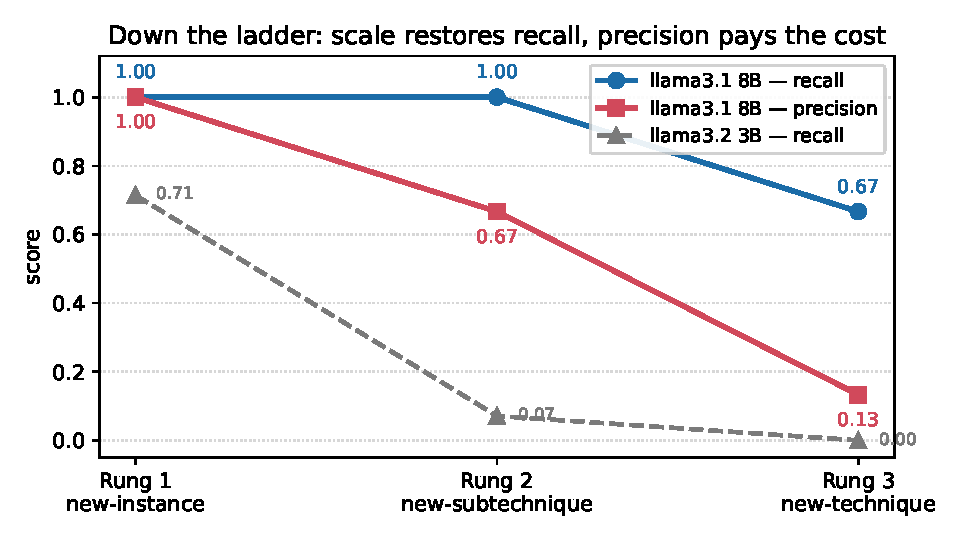
\includegraphics[width=\columnwidth]{fig-ladder}
\caption{Down the ladder. The 3B model's recall collapses with distance
($0.71\!\rightarrow\!0.07\!\rightarrow\!0.00$); the 8B model holds recall
($1.00\!\rightarrow\!1.00\!\rightarrow\!0.67$) but its precision falls
($1.00\!\rightarrow\!0.67\!\rightarrow\!0.13$). Generalization is a
precision/recall frontier that shifts with scale, not a cliff.}
\label{fig:ladder}
\end{figure}

\begin{table}[t]
\caption{Scale: 3B vs.\ 8B (best of zero/few recall; precision at that point).}
\label{tab:scale}
\small
\begin{tabular}{@{}lrrr@{}}
\toprule
Rung & 3B recall & 8B recall & 8B precision \\
\midrule
1 new-instance     & 0.71 & \textbf{1.00} & 1.00 \\
2 new-subtechnique & 0.07 & \textbf{1.00} & 0.67 \\
3 new-technique    & 0.00 & \textbf{0.67} & 0.13 \\
\bottomrule
\end{tabular}
\end{table}

Scaling 3B $\rightarrow$ 8B overturns the collapse (Table~\ref{tab:scale}):
recall rises at every rung and 8B recognizes the injection primitive 3B missed.
The cost moves to \emph{precision}, which falls with ladder distance
($1.00\!\rightarrow\!0.67\!\rightarrow\!0.13$): 8B transfers by becoming a broad,
trigger-happy detector that flags ordinary process-access handles
(\texttt{svchost}$\rightarrow$\texttt{svchost}) to catch the real attacks.
Few-shot is \emph{directional}: same-family exemplars raise NTDS precision
($0.26\!\rightarrow\!0.67$) while holding recall, but off-target T1003 exemplars
\emph{destroy} injection recall ($0.67\!\rightarrow\!0.00$) by anchoring the
model to credential dumping. Figure~\ref{fig:ladder} summarizes the two trends:
recall rising with scale, precision falling with ladder distance.

\section{Discussion and Limitations}
\label{sec:discussion}
Neither family is a general detector. The invariant is a precise, narrow sensor
that must be rebuilt per surface; the LLM at scale is a broad, shallow one whose
generality is partly lexical and whose precision decays off-distribution. The
contribution is the \emph{map}: where each sits on the ladder.
\textbf{Limitations.} Small attack-event counts per rung (7/14/3) make recall
coarse; LLM precision is on benign subsamples; ground truth is a derived rule;
models are 3B/8B local, not frontier/tool-calling---the \emph{shape} (recall
rises with scale, precision falls with distance) is the claim, not exact values.

\section{Conclusion and Future Work}
\label{sec:conclusion}
We measured detection generalization as distance on an ATT\&CK ladder and found
it bounded by the telemetry surface and intent, with a scale-dependent
precision/recall frontier. Future: a new-\emph{chain} rung (multi-step OTRF
\texttt{apt29}/\texttt{Log4Shell}); a frontier/tool-calling LLM; and closing the
loop with the released co-evolution engine---an adaptive Red that mutates
tool/access to evade a learning Blue---run against the measured ladder.

\bibliographystyle{ACM-Reference-Format}
\bibliography{references}

\end{document}
